`\section{Lecture 5 | Model Free Control}

\subsubsection*{Off and On Policy Learning}
\begin{itemize}
  \item On Policy Learning - Learn about policy \(\pi \) from experience sampled from \(\pi \).
  \item Off Policy Learning - Learn about policy \(\pi \) from experience sampled from \(\mu \).
\end{itemize}

\subsection{On Pilocy Monte Carlo Control}

\begin{figure}[H]
    \begin{minipage}{0.5\textwidth}
        \begin{itemize}
            \item Policy Evaluation - Estimate \(v_\pi \) e.g. Iterative Policy Evaluation. 
            \item Policy Improvement - Generate \(\pi' \geq \pi \) e.g. Greedy Policy Improvement.
          \end{itemize}
    \end{minipage}%
    \begin{minipage}{0.5\textwidth}
      % Your image goes here
      \centering
      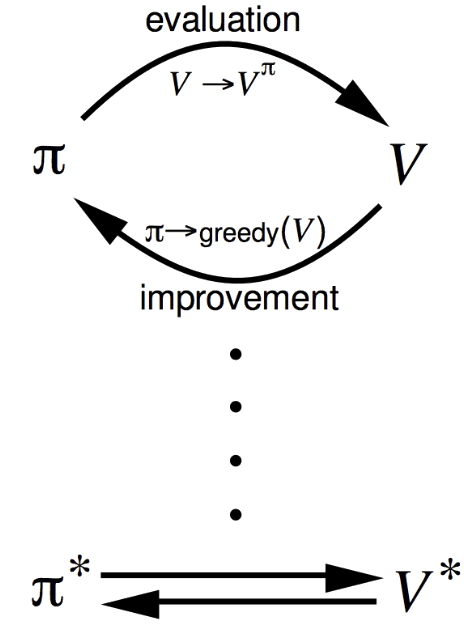
\includegraphics[height=0.75\textwidth]{figures/gpi.png}
      \caption{Generalised Policy Iteration}
        \label{fig:gpi}
    \end{minipage}
  \end{figure}

One of the simple ideas is to use Monte Carlo Policy Evaluation and Greedy Policy Improvement.
BUt this quickly runs into problems:
\begin{itemize}
  \item Policy Evaluation - Monte Carlo Policy Evaluation with value function, requires
  the model of the MDP.
  \item Policy Improvement - Greedy Policy Improvement faces the issue of the
  expectation of the entire state space.
\end{itemize}
So, greefy policy improvemnent over \(V(s)\) requires model of the MDP.
\[
  \pi'(s) = \argmax_{a \in \mathcal{A}(s)} \mathcal{R}^a_s + \mathcal{P} ^a_{ss'} V(s')
\]
replacing the value function with stae action value function, the policy evaluation is model
free.
\[
  \pi'(s) = \argmax_{a \in \mathcal{A}(s)} Q(s,a)
\]

\subsubsection{\(\epsilon\)-Greedy Exploration}
This is one of the simplest ways to explore the state space. The idea is to choose the greedy
action with probability \(1-\epsilon\) and a random action with probability \(\epsilon\). 
Thus all \(m\) actions have a non-zero probability of being selected. 
\[
  \pi(a|s) = \begin{cases}
    1-\epsilon + \frac{\epsilon}{m} & \text{if } a^{\star}  = \argmax\limits_
    {a \in \mathcal{A}(s)} Q(s,a) \\
    \frac{\epsilon}{m} & \text{otherwise}
  \end{cases}
\]


\begin{theorem}[\(\epsilon \)-Greedy Policy Improvement]
  For any \(\epsilon \)-greedy policy \(\pi\), the \(\epsilon \)-greedy policy \(\pi'\) with
  respect to \(q_\pi \) is an improvement, \(v_{\pi'}(s) \geq v_\pi(s)\).
\end{theorem}
\begin{proof}
  \begin{align*}
    q_\pi(s, \pi'(s)) &= \sum_{a \in \mathcal{A}(s)} \pi'(a|s) q_\pi(s,a) \\
    &= \frac{\epsilon}{m} \sum_{a \in \mathcal{A}(s)} q_\pi(s,a) + (1-\epsilon) \max_{a \in
    \mathcal{A}(s)} q_\pi(s,a) \\
    &\geq \frac{\epsilon}{m} \sum_{a \in \mathcal{A}(s)} q_\pi(s,a) + (1-\epsilon) \sum_{a
    \in \mathcal{A}(s)} \frac{\pi(a|s) - \frac{\epsilon}{m}}{1-\epsilon} q_\pi(s,a) \\
    &= \sum_{a \in \mathcal{A}(s)} \pi(a|s) q_\pi(s,a) = v_\pi(s)
  \end{align*}
  Therefore from policy improvement theorem, \(v_{\pi'}(s) \geq v_\pi(s)\).
\end{proof} 

Thus the Monte Carlo Control can be summarissed as follows:
\begin{figure}[H]
  \begin{minipage}{0.5\textwidth}
    Every episode:
      \begin{itemize}
          \item Policy Evaluation - Monte Carlo Policy Evaluation with value function : 
          \(Q \approx q_\pi \) 
          \item Policy Improvement - \(\epsilon \)-Greedy Policy Improvement.
        \end{itemize}
  \end{minipage}%
  \begin{minipage}{0.5\textwidth}
    % Your image goes here
    \centering
    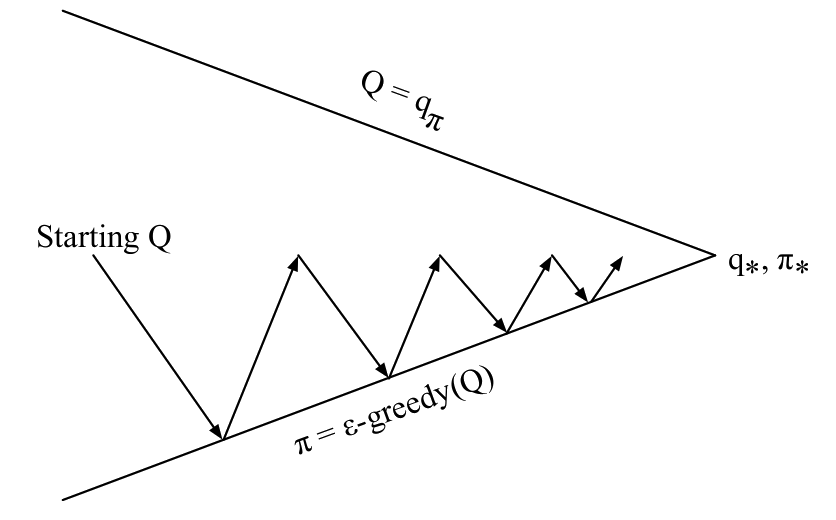
\includegraphics[width=\textwidth]{figures/mc-eps.png}
    \caption{Monte Carlo Control}
    \label{fig:mc-eps}
  \end{minipage}
\end{figure}

\subsubsection{GLIE}
GLIE = Greedy in the Limit with Infinite Exploration.

\begin{theorem}[Greedy in the Limit with Infinite Exploration]
  If all state-action pairs are explored infinitely many times, then the policy converges
  to a greedy policy, \(\lim_{k \to \infty} \pi_k(a|s) = \mathbb{1}(a = \argmax_{a \in
  \mathcal{A}(s)} Q(s,a))\).
  Thus, GLIE has these two properties:
  \begin{itemize}
    \item Every state-action pair is visited infinitely many times.
    \[
      \lim_{k \to \infty} N_k(s,a) = \infty
    \]
    \item The policy converges on a greedy policy.
    \[
      \lim_{k \to \infty} \pi_k(a|s) = \bm{1}(a = \argmax_{a \in \mathcal{A}(s)} Q(s,a))
    \]
  \end{itemize}
\end{theorem}
For example, \(\epsilon\)-greedy with \(\epsilon = \frac{1}{k}\) for the \(k^{th}\) episode
satisfies GLIE.

\subsubsection{GLIE Monte Carlo Control}
The algortihm can be described as:
\begin{itemize}
  \item Sample \(k^{th}\) episode using \(\pi_k\): \(S_0, A_0, R_1, \dots, S_{T}\)
  \item For each state \(S_t\) and action \(A_t\) in the episode:
  \[
    \begin{aligned}
      N(S_t, A_t) &\leftarrow N(S_t, A_t) + 1 \\
      Q(S_t, A_t) &\leftarrow Q(S_t, A_t) + \frac{1}{N(S_t, A_t)} (G_t - Q(S_t, A_t)) \\
      \pi(S_t) &\leftarrow \argmax_{a \in \mathcal{A}(S_t)} Q(S_t, a)  
    \end{aligned}
  \]
  \item Improve the policy based on new action value function.
  \[
    \begin{aligned}
      \epsilon &\leftarrow \frac{1}{k} \\
      \pi &\leftarrow \epsilon\text{-greedy}(Q)
    \end{aligned}
  \]
\end{itemize}
\begin{theorem}[Convergence of GLIE Monte Carlo Control]
  GLIE Monte Carlo Control converges to the optimal action-value function, \(Q(s,a) \to
  q_\star(s,a)\).
\end{theorem}

\subsection{SARSA(\(\lambda \))}
Use the natureal idea to replace MC wtth TD(\(\lambda\)). So we will be applying,
TD to the action value function, \(Q(s,a)\), by using the \(\epsilon\)-greedy policy
improvement. The policy is updated at every time step.

Thus at every time step:
\begin{itemize}
  \item Policy Evaluation - SARSA(\(\lambda\)) : \(Q \approx q_\pi \)
  \[
    Q(S,A) \leftarrow Q(S,A) + \alpha \left( 
      R + \gamma Q(S', A') - Q(S,A)
    \right) 
  \]
  \item Policy Improvement - \(\epsilon\)-Greedy Policy Improvement.
\end{itemize}
The algorithm for SARSA is shown in \autoref{alg:sarsa}.
\begin{algorithm}[H]
  \caption{SARSA}
  \label{alg:sarsa}
  \begin{algorithmic}[1]
    \State Initialise \(Q(s,a)\) arbitrarily and \(E(s,a) = 0\) for all \(s \in \mathcal{S},
    a \in \mathcal{A}(s)\)
    \State Q(terminal-state, \(\cdot\)) = 0
    \For{each episode}
      \State Initialise \(S\)
      \State Choose \(A\) from \(S\) using policy derived from \(Q\) (e.g.
      \(\epsilon\)-greedy)
      \For{each step of episode}
        \State Take action \(A\), observe \(R, S'\)
        \State Choose \(A'\) from \(S'\) using policy derived from \(Q\) (e.g.
        \(\epsilon\)-greedy)
        \State \(Q(s,a) \leftarrow Q(s,a) + \alpha \left[ 
          R + \gamma Q(S', A') - Q(S,A)
        \right] \)
        \State \(S \leftarrow S'\), \(A \leftarrow A'\)
      \EndFor
    \EndFor
  \end{algorithmic}
\end{algorithm}

\begin{theorem}[Convergence of SARSA]
  SARSA converges to the optimal action-value function, \(Q(s,a) \to q_\star(s,a)\), under
  the following conditions:
  \begin{itemize}
    \item GLIE sequence of policies \(p_t(a|s)\) 
    \item Robbins-Monro sequence of step-sizes
    \[
      \begin{aligned}
        \sum_{t=1}^{\infty} \alpha_t(s,a) &= \infty \\
        \sum_{t=1}^{\infty} \alpha_t^2(s,a) &< \infty
      \end{aligned}
    \]
    The first equation ensures that the steps are large enough to overcome the initial
    conditions and the second equation ensures that the steps are small enough to converge.

  \end{itemize}
\end{theorem}
\subsubsection{\(n\)-step SARSA}
Similar to n-step TD, we can also define \(n\) -step SARSA. Consider the following \(n\)-step
returns for \(n \geq 1\):
\[
  \begin{aligned}
    n &= 1 \implies q_t^{(1)} = R_{t+1} + \gamma Q(S_{t+1}, A_{t+1}) && \text{SARSA} \\
    n &= 2 \implies q_t^{(2)} = R_{t+1} + \gamma R_{t+2} + \gamma^2 Q(S_{t+2}, A_{t+2}) \\
    \vdots & \vdots \\
    n &= \infty \implies q_t^{(\infty)} = R_{t+1} + \gamma R_{t+2} + \dots + \gamma^{T-t-1}
    && \text{Monte Carlo}
  \end{aligned}
\]
with the \(n\)-step Q-return being defined as:
\[
  q_t^{(n)} = R_{t+1} + \gamma R_{t+2} + \dots + \gamma^{n-1} R_{t+n} + \gamma^n Q(S_{t+n},
  A_{t+n})
\]
The \(n\)-step SARSA updates \(Q(s,a)\) towards \(n\)-step Q-retuen as follows:
\[
  Q(S_t, A_t) \leftarrow Q(S_t, A_t) + \alpha \left[ 
    q_t^{(n)} - Q(S_t, A_t)
  \right]
\]
\subsubsection{SARSA(\(\lambda\))}
Similar to TD(\(\lambda\)), we can also define SARSA(\(\lambda\)). 

The \(q^\lambda\) return combines all the \(n\)-step Q-returns \(q_t^{(n)}\) using 
exponential weighting, with the weights summing to 1.
\[
  q_t^\lambda = (1-\lambda) \sum_{n=1}^{\infty} \lambda^{n-1} q_t^{(n)}
\]  
Thus, the Forward View of SARSA(\(\lambda\)) is given by:
\[
  Q(S_t, A_t) \leftarrow Q(S_t, A_t) + \alpha \left[ 
    q_t^\lambda - Q(S_t, A_t)
  \right]
\]
\subsubsection*{Forward View of SARSA(\(\lambda\))}
The \(q^\lambda\) return combines all the \(n\)-step Q-returns \(q_t^{(n)}\) using 
exponential weighting, with the weights summing to 1.
\[
  q_t^\lambda = (1-\lambda) \sum_{n=1}^{\infty} \lambda^{n-1} q_t^{(n)}
\] 

\begin{figure}[H]
  \centering
  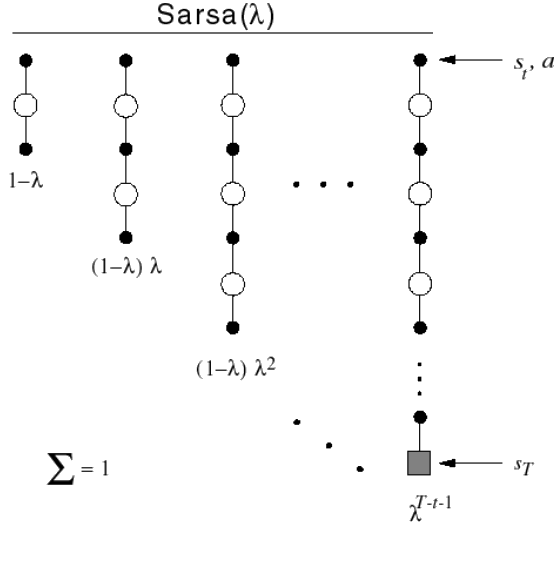
\includegraphics[width=0.75\textwidth]{figures/fv-srasa.png}
  \caption{Forward View of SARSA(\(\lambda\))}
  \label{fig:fv-srasa}
\end{figure}

\subsubsection*{Backward View of SARSA(\(\lambda\))}
Similar to TD(\(\lambda\)), we can also define SARSA(\(\lambda\)) using eligibility traces.
It is important to note that SARSA(\(\lambda \)) has one eligibility trace for each
state-action pair, \(E_t(s,a)\). The eligibility trace is updated as follows:
\[
  \begin{aligned}
    E_0(s,a) &= 0 \\
    E_t(s,a) &= \gamma \lambda E_{t-1}(s,a) + \bm{1}(S_t = s, A_t = a)
  \end{aligned}
\]
Tus, \(Q(s,a)\) is updates for wevery state \(s\) and action \(a\) in proportion to the TD
error \(\delta _t\) and the eligibility trace \(E_t(s,a)\).
\[
  \begin{aligned}
    \delta _t &= R_{t+1} + \gamma Q(S_{t+1}, A_{t+1}) - Q(S_t, A_t) \\
    Q(s,a) &\leftarrow Q(s,a) + \alpha \delta _t E_t(s,a)
  \end{aligned}
\]
Thus,the SARSA(\(\lambda\)) algorithm is given by:
\begin{algorithm}[H]
  \caption{SARSA(\(\lambda\))}
  \label{alg:sarsa-lambda}
  \begin{algorithmic}[1]
    \State Initialise \(Q(s,a)\) and \(E(s,a) = 0\) for all \(s \in \mathcal{S}, a \in
    \mathcal{A}(s)\)
    \For{each episode}
      \State Initialise \(S\)
      \State Choose \(A\) from \(S\) using policy derived from \(Q\) (e.g.
      \(\epsilon\)-greedy)
      \State \(E(S,A) = 0 \forall S \in \mathcal{S}, A \in \mathcal{A}(S)\)
      \For{each step of episode}
        \State Take action \(A\), observe \(R, S'\)
        \State Choose \(A'\) from \(S'\) using policy derived from \(Q\) (e.g.
        \(\epsilon\)-greedy)
        \State \(\delta \leftarrow R + \gamma Q(S', A') - Q(S,A)\)
        \State \(E(S,A) \leftarrow E(S,A) + 1\)
        \For{all \(s \in \mathcal{S}, a \in \mathcal{A}(s)\)}
          \State \(Q(s,a) \leftarrow Q(s,a) + \alpha \delta E(s,a)\)
          \State \(E(s,a) \leftarrow \gamma \lambda E(s,a)\)
        \EndFor
        \State \(S \leftarrow S'\), \(A \leftarrow A'\)
      \EndFor
    \EndFor
  \end{algorithmic}
\end{algorithm}

\subsection{Off Policy Learning}
In off policy learning, we evaluate target policy \(\pi(a|s)\) to compute \(v_\pi(s)\) or \(q_\pi
(s,a)\) using followiong the behaviour poliicy \(\mu(a|s)\)
\[
  \{  S_1, A_1, R_2, \dots, S_T \} \sim \mu
\]
This allows us to learn about the optimal policy \(\pi_\star\) fromobserving humans 
or other agents. Experience generated from old policies \(\pi _1, \pi _2, \dots, \pi _{t-1}\)
can be reused to learn about the current policy \(\pi _t\). Off policy learning allows us to
learn about multiple policies simultaneously while only following one policy. It also allows
us to learn about the optimal policy while following an exploratory policy. 

\subsubsection{Importance Sampling}
Estimate the expectation of a different distribution:
\[
  \begin{aligned}
    \mathbb{E}_{x \sim p}[f(x)] &= \sum_{x} p(x) f(x) \\
    &= \sum_{x} q(x) \frac{p(x)}{q(x)} f(x) \\
    &= \mathbb{E}_{x \sim q} \left[ 
      \frac{p(x)}{q(x)} f(x)
    \right]    
  \end{aligned}
\]
\begin{note}
  Wathc this youtube video for a better understanding of importance sampling:
  \href{https://www.youtube.com/watch?v=C3p2wI4RAi8}{Importance Sampling}
\end{note}

\subsubsection{Imnporatnce Sampling for Off Policy Monte Carlo}
Imporatnce Sampling in Monte Carlo off policy learning uses the retuends generated 
from \(\mu\) to evaluest teh policy \(\pi\). The returns are weighted by the similarity
between two policies.

Mulitplying the importance sampling corrections along the whole episode, we get:
\[
  \begin{aligned}
    G_t^{\pi/\mu}  &= R_{t+1} + \gamma R_{t+2} + \dots + \gamma^{T-t-1} R_{T} \\
    &= \frac{\pi(A_t|S_t)}{\mu(A_t|S_t)} \frac{\pi(A_{t+1}|S_{t+1})}{\mu(A_{t+1}|S_{t+1})}
    \dots \frac{\pi(A_{T-1}|S_{T-1})}{\mu(A_{T-1}|S_{T-1})} G_t^\mu
  \end{aligned}
\]
Updating the value towards the corrected return, we get:
\[
  V(S_t) \leftarrow V(S_t) + \alpha \left[ 
    G_t^{\pi/\mu} - V(S_t)
  \right]
\]
Important point to note that the importance sampling cannot be used if \(\mu =0\) when 
\(\pi \neq 0\). Also, imporatnce sampling can increase the variance of the returns. And in
practice the Monte Carlo off policy learning is not used and is a really bad idea.

\subsubsection{Off Policy TD Learning}
Similar to off policy Monte Carlo, we can also define off policy TD learning. The idea is
as follows:

\begin{itemize}
  \item Use TD target generated from \(\mu\) to evaluate \(\pi\).
  \item Weight the TD target by the similarity between two policies given by the importance
  sampling.
  \item Thus we only need singel importave sampling correction:
  \[
    V(S_t) \leftarrow V(S_t) + \alpha \left[
    \frac{\pi(A_t|S_t)}{\mu(A_t|S_t)} \left( 
      R_{t+1} + \gamma V(S_{t+1}) - V(S_t)
    \right) 
    \right]
  \]
\item Thisi methiod has much lower varianvce compared to the Monte Carlo off policy learning.
\item The plocies only need to be siliar over a single time step
\end{itemize}

\subsection{Q-Learning}
Consider the off policy learning of action values \(Q(s,a)\). This is specific to TD(0).
To make use of thew action values to do off policy learning to avoid the use of importance
sampling.

The next action is chosen using behaviour policy \(A_{t+1} \sim \mu(\cdot|S_{t})\). 
But we also consider alternative successort action \(A' \sim \pi(\cdot|S_{t+1})\),
and update \(Q(S_t,A_t)\) towards the value of the alternative successor action:
\[
    Q(S_t, A_t) \leftarrow Q(S_t, A_t) + \alpha \left[ 
      R_{t+1} + \gamma Q(S_{t+1}, A') - Q(S_t, A_t)
    \right]
\]

\subsubsection{Off Policy control with Q-Learning}
We allow both the behaviour and the target policies to improve. So the target policy
\(\pi\) is greedy wrt \(Q)s,a\)
\[
  \pi(S_{t+1}) = \argmax_{a^{\prime}} Q(S_{t+1}, a^{\prime})
\]
and the behaviour policy \(\mu\) is \(\epsilon\)-greedy wrt \(Q(s,a)\)
Thus, behaiour plociy is also goint to explore the part of the state space that the target
policy is not exploring. Thus, the Q-learning target then simplifies to:
\[
  \begin{aligned}
    R_{t+1} + \gamma Q(S_{t+1}, A') &= R_{t+1} + \gamma Q(S_{t+1}, \argmax_{a^{\prime}}
    Q(S_{t+1}, a^{\prime})) \\
    &= R_{t+1} + \gamma \max_{a^{\prime}} Q(S_{t+1}, a^{\prime})  
  \end{aligned}
\]
Thus, the Q-learning update is given by:
\begin{figure}[H]
  \begin{minipage}{0.5\textwidth}
    \[
      Q(S,A) \leftarrow Q(S,A) + \alpha \left[ 
        R + \gamma \max_{a^{\prime}} Q(S', a^{\prime}) - Q(S,A)
      \right]
    \]
  \end{minipage}%
  \begin{minipage}{0.5\textwidth}
    % Your image goes here
    \centering
    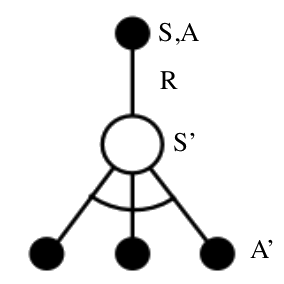
\includegraphics[width=0.4\textwidth]{figures/sarsamax.png}
    \caption{Q-Learning (SARSA max)}
    \label{fig:sarsamax}
  \end{minipage}
\end{figure}
\begin{theorem}[Convergence of Q-learning]
  Q-learning control converges to the optimal action-value function, \(Q(s,a) \to q_\star(s,a)\),
\end{theorem}
The algorith for Q-learning is given by:
\begin{algorithm}[H]
  \caption{Q-learning}
  \label{alg:q-learning}
  \begin{algorithmic}[1]
    \State Initialise \(Q(s,a) \forall s \in \mathcal{S}, a \in \mathcal{A}(s)\) arbitrarily.
    \For{each episode}
      \State Initialise \(S\)
      \For{each step of episode}
        \State Choose \(A\) from \(S\) using policy derived from \(Q\) (e.g.
        \(\epsilon\)-greedy)
        \State Take action \(A\), observe \(R, S'\)
        \State \(Q(S,A) \leftarrow Q(S,A) + \alpha \left[ 
          R + \gamma \max_{a^{\prime}} Q(S', a^{\prime}) - Q(S,A)
        \right] \)
        \State \(S \leftarrow S'\)
      \EndFor
    \EndFor
  \end{algorithmic}
\end{algorithm}

\subsection{Relationship between DP and TD}
\begin{table}[H]
  \centering
  \begin{tabular}{cc}
      \toprule
      Full Backup(DP) &  Sample Backup(TD) \\
    \midrule
       Iterative Policy Evaluation  & TD learning   \\
       \(V(s) \gets \mathbb{E} \left[ 
         R + \gamma V(S') | s 
        \right] \) & \(V(S) \overset{\alpha}{\gets} R + \gamma V(S')\) \\
        \hline
        Q-Policy Iteration & Q-learning \\
        \(Q(s,a) \gets \mathbb{E} \left[ 
          R + \gamma Q(S', a^{\prime}) | s,a
        \right] \) & \(Q(S,A) \overset{\alpha}{\gets} R + \gamma Q(S', A^{\prime})\) \\
        \hline
        Q-Value Iteration & Q-learning \\
        \(Q(s,a) \gets \mathbb{E} \left[ 
          R + \gamma \max\limits_{a^{\prime}\in \mathcal{A} } Q(S', a^{\prime}) | s,a
        \right] \) & \(Q(S,A) \overset{\alpha}{\gets} R + \gamma 
        \max\limits_{a^{\prime}\in \mathcal{A} } Q(S', A^{\prime})\) \\
      \bottomrule
  \end{tabular}
\caption{Relationship between DP and TD}
  \label{tab:dp-td}
\end{table}
where \(x \overset{\alpha}{\gets} y\) means \(x \leftarrow x + \alpha (y-x)\). 